\section{Существующие системы управления базами данных по модели данных}

\subsection{Обзор СУБД по модели данных}

В данном разделе рассмотрены существующие СУБД по модели данных, которые используются в настоящее время. Все они различаются по своим особенностям и применяемым технологиям.

\subsubsection{Иерархическая СУБД}
В иерархической модели данных используется представление базы данных в виде древовидной структуры, состоящей из объектов различных уровней \cite{adreyev}.

В моделях данных, где устанавливаются отношения предок-потомок, каждый объект может содержать несколько объектов более низкого уровня.
Эти отношения образуют иерархическую структуру данных, где один объект является предком для другого объекта, который является его потомком.
При этом, в иерархической модели данных каждый объект-потомок может иметь только одного предка.
Это означает, что объект-потомок находится в строгом отношении с одним объектом-предком.
Однако, объект предок может иметь несколько объектов-потомков, что позволяет создавать ветвистую иерархию.

Иерархические СУБД применяются в ситуациях, когда данные естественным образом организованы в иерархическую структуру.

К преимуществам иерархическая СУБД относят:
\begin{itemize}
	\item быстрый и эффективный поиск данных;
	\item легко добавлять/удалять информацию;
	\item эффективное хранение данных;
	\item производительность.
\end{itemize}

Недостатками таких моделей являются:
\begin{itemize}
	\item ограниченная гибкость;
	\item сложно поддерживать и обновлять;
	\item ограниченная поддержка манипулирования данными;
	\item ограниченная совместимость;
	\item отсутствие стандартизации.
\end{itemize}

Файловая система представлена на рисунке \ref{img:pic1}.
\begin{figure}[h!]
	\centering
	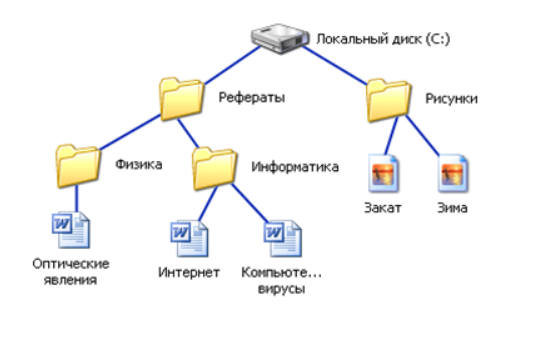
\includegraphics[height=0.3\textheight]{img/pic1} % height
	\caption{Файловая система}
	\label{img:pic1}
\end{figure}

\subsubsection{Сетевая СУБД}

Сетевая модель данных является расширением иерархической модели, предоставляя более гибкие возможности для организации данных и установления связей между записями \cite{instument}.

В сетевой модели каждый потомок может иметь несколько предков, в отличие от иерархической модели, где каждый потомок имеет только одного предка.
Это позволяет создавать сложные и перекрестные связи между записями, что способствует более гибкому представлению и организации данных.
Сетевая база данных состоит из двух основных компонентов: экземпляров записей и экземпляров связей.
Каждый экземпляр связи определяет отношение между экземпляром предка и одним или несколькими экземплярами потомка.
Экземпляр связи содержит ссылку на экземпляр предка и упорядоченный набор ссылок на экземпляры потомка.

Сетевая архитектура представлена на рисунке \ref{img:pic2}.
\begin{figure}[h!]
	\centering
	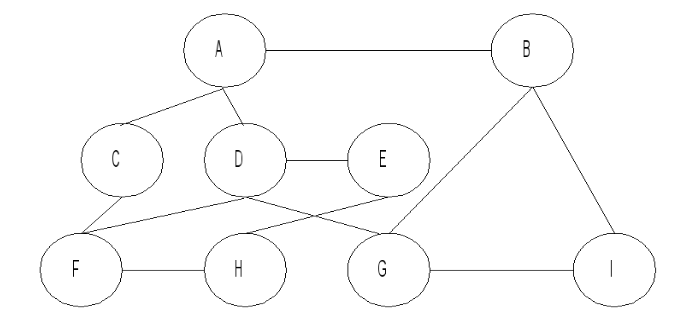
\includegraphics[height=0.3\textheight]{img/pic2} % height
	\caption{Сетевая модель данных}
	\label{img:pic2}
\end{figure}

К преимуществам cетевая СУБД относят \cite{setevaya}:
\begin{itemize}
	\item обработка больших объемов информации (возможность построения на основе таких СУБД «хранилищ данных»);
	\item поддержка аналитической обработки данных;
	\item эффективная реализация обработки данных по показателям затрат памяти и оперативности.
\end{itemize}

Недостатками таких моделей являются \cite{setevaya}:
\begin{itemize}
	\item высокая сложность и жесткость схемы БД, построенной на ее основе;
	\item сложность для понимания и выполнения обработки информации в БД обычным пользователем;
	\item ослаблен контроль целостности связей вследствие допустимости установления произвольных связей между записями;
\end{itemize}

\subsubsection{Реляционные БД}
Реляционная база данных --- это набор данных с предопределенными отношениями между ними.
Эти данные организованы в виде набора таблиц, состоящих из столбцов и строк.
Таблицы хранят информацию об объектах, представленных в базе данных.
Таблицы состоят из строк --- записей и столбцов --- полей.
Каждый столбец таблицы хранит определенный тип данных, каждая ячейка содержит значение атрибута.
Каждая строка в таблице может быть помечена уникальным идентификатором, называемым первичным ключом, а строки из нескольких таблиц могут быть связаны с помощью внешнего
ключа.
Доступ к этим данным можно получить многими способами без реорганизации таблиц базы данных \cite{relation}.

Реляционная модель является удобной и наиболее широко используемой формой представления данных.
Широко распространенной реляционной СУБД является программа фирмы Microsoft Access \cite{instument}. Специальные программы класса СУБД (Oracle, MS SQL, Adabas, Informix, MySQL, SQlite и
др.) разрабатываются таким образом, чтобы предоставлять пользователям широкие возможности их развития.

Преимуществами такой модели являются \cite{relation2}:
\begin{itemize}
	\item структурированность и организация данных;
	\item целостность данных;
	\item гибкий язык запросов;
	\item поддержка транзакций и согласованности;
	\item удобство администрирования;
	\item безопасность данных.
\end{itemize}

Недостатками реляционной модели являются \cite{instument}:
\begin{itemize}
	\item невысокую эффективность;
	\item возможность обеспечения быстрого поиска с помощью индексов.
\end{itemize}

\subsection{Критерии сравнения систем управления базами данных}

В данном разделе описаны критерии, которые используются для выбора
СУБД при создании информационных систем.

\begin{table}[h]
	\begin{center}
		\begin{threeparttable}
			\captionsetup{justification=raggedright,singlelinecheck=off}
			\caption{Критерии выбора СУБД \cite{one}}
			\label{tbl:time_even}
			\begin{tabular}{|c|c|}
				\hline
				Критерий & Описание\\
				\hline Моделирование данных & Используемая модель данных\\	
				\hline \makecell{Особенности архитектуры \\ и функциональные возможности} & \makecell{Мобильность, Масштабируемость, \\Распределенность, \\Сетевые возможности}\\
				\hline Контроль работы системы & \makecell{Контроль использования \\ памяти компьютера}\\
				\hline Производительность & \makecell{Оценивает скорость выполнения\\запросов и обработки данных}\\
				\hline Надежность & \makecell{Связана с устойчивостью системы\\к сбоям, ее способностью \\обеспечивать доступность данных}\\
				\hline Требования к рабочей среде & \makecell{определяют условия, под которыми\\ СУБД должна функционировать}\\\hline
			\end{tabular}
		\end{threeparttable}
	\end{center}
\end{table}

\subsection{Сравнение систем управления базами данных}
В данном разделе описаны все описанные СУБД, а также дано сравнение этих СУБД по всем критериям, указанным в таблице \ref{tbl:time_even}.
\begin{table}[h]
	\begin{center}
		\begin{threeparttable}
			\captionsetup{justification=raggedright,singlelinecheck=off}
			\caption{Сравнение СУБД}
			\label{tbl:table1}
			\begin{tabular}{|c|c|c|c|}
				\hline
				&\multicolumn{3}{c|}{\bfseries СУБД} \\\cline{2-4}
				Критерий & Иерархическая & Сетевая & Реляционная\\
				\hline \makecell{Моделирование\\ данных} & \makecell{Иерархическая\\структура,\\древовидная\\ организация}& \makecell{Сетевая\\структура,\\разрешает\\несколько\\родителей}& \makecell{Табличная\\структура,\\данные\\представлены\\в таблицах}\\	
				\hline \makecell{Особенности\\архитектуры  и\\функциональные\\возможности} & \makecell{Простая, но\\ограниченная в\\ функциональности} &\makecell{Более гибкая\\ архитектура\\ с поддержкой\\ нескольких\\ родительских\\связей}&\makecell{Сложные\\запросы\\через язык\\SQL,\\ интерфейс}\\
				\hline \makecell{Контроль\\работы системы} &\makecell{Ограниченный\\контроль,\\сложно обеспечить\\целостность}&\makecell{Более\\гибкий\\контроль, но\\сложность\\ управления}&\makecell{Эффективный\\контроль\\через\\язык SQL и\\ограничения}\\
				\hline \makecell{Производи-\\тельность} &\makecell{Зависит от\\структуры и\\запросов,\\может быть\\эффективной для\\определенных\\задач}&\makecell{Улучшенная\\для некоторых\\сценариев}&\makecell{Эффективные\\операции с\\использованием\\индексов,\\ оптимизи-\\рованные\\для чтения\\данных} \\
				\hline Надежность &\makecell{Ограниченная\\надежность\\из-за\\ограничений\\ структуры}&\makecell{Улучшенная\\надежность\\с гибкостью\\в построении\\ связей}&\makecell{Высокая\\надежность\\через\\использование\\транзакций\\и ограничений\\ целостности}\\
				\hline \makecell{Требования\\к рабочей среде} &\makecell{Зависит от\\конкретной\\реализации\\и объема\\данных}&\makecell{Зависит от\\конкретной\\реализации\\и структуры}&\makecell{Обширные\\ требования\\к хранению\\и обработке\\данных}\\\hline
			\end{tabular}
		\end{threeparttable}
	\end{center}
\end{table}
\clearpage
Из проведенного сравнения видно, что каждый тип СУБД имеет свои особенности и подходит для определенных сценариев использования.

\begin{itemize}
	\item Моделирование данных:
	\begin{itemize}
		\item Иерархическая и сетевая СУБД подходят для данных с явной структурой, где важны отношения и иерархии;
		\item Реляционная СУБД эффективна для хранения данных в табличной форме, обеспечивая стандартизацию;
	\end{itemize}
	\item Контроль работы системы:
	\begin{itemize}
		\item Реляционная СУБД выделяется эффективным контролем через SQL и поддержкой транзакций;
	\end{itemize}
	\item Особенности архитектуры и функциональные возможности:
	\begin{itemize}
		\item Сетевая СУБД предоставляет более гибкую архитектуру, поддерживая несколько родительских связей;
		\item Реляционная СУБД отличается стандартизированным интерфейсом и поддержкой сложных SQL-запросов;
	\end{itemize}
	\item Производительность и надежность:
	\begin{itemize}
		\item Иерархическая и сетевая СУБД подходят для специфических сценариев, их производительность зависит от структуры и запросов;
		\item Реляционная СУБД выделяется высокой производительностью и надежностью за счет эффективных операций и поддержки ACID;
	\end{itemize}
	\item Требования к рабочей среде:
	\begin{itemize}
		\item Реляционная СУБД требует обширных ресурсов для хранения и обработки данных;
		\item Иерархическая и сетевая СУБД управляются более удобно, но с ограничениями структуры.
	\end{itemize}
\end{itemize}
Итак, выбор типа СУБД зависит от конкретных требований проекта, структуры данных и предполагаемых сценариев использования.
\clearpage
\section{Существующие системы управления базами данных по способу доступа к базе данных}
\subsection{Обзор СУБД по способу доступа к базе данных}
\subsubsection{Файл-серверные}
В файл-серверных СУБД файлы данных располагаются централизованно на файл-сервере \cite{adreyev}. Возможна многопользовательская работа с одной и той же БД, когда каждый пользователь со своего компьютера запускает приложение, расположенное на сетевом сервере. 
Тогда на компьютере пользователя запускается копия приложения. В архитектуре файл-сервер вся тяжесть выполнения запросов к базе данных и управления целостностью базы данных ложится на приложение пользователя.
По каждому запросу к БД из приложения данные из таблиц БД
перегоняются на компьютер пользователя, независимо от того, сколько реально нужно данных для
выполнения запроса. После этого выполняется запрос. Каждый пользователь имеет на своем компьютере
локальную копию данных.
На каждом клиентском компьютере (рабочей станции) располагается СУБД, который время от времени обновляет из реальной БД, расположенной на сетевом сервере.
На данный момент файл-серверная технология считается устаревшей.

Такая архитектура имеет следующие преимущества \cite{classichoose}:
\begin{itemize}
	\item низкая стоимость разработки, высокая скорость разработки;
	\item недорогой вариант для многопользовательской одновременной работы;
	\item невысокая стоимость обновления и изменения программного обеспечения.
\end{itemize}

Однако у архитектуры файл-сервер есть ряд недостатков \cite{classichoose}:
\begin{itemize}
	\item рост числа клиентов резко увеличивает объем трафика и нагрузку на сети
	передачи данных;
	\item высокие затраты на сопровождение сервисов бизнес-логики на каждой
	клиентской рабочей станции;
	\item низкая надежность системы.
\end{itemize}

На рисунке \ref{img:filesever} приведена файл-серверная архитектура.
\begin{figure}[h!]
	\centering
	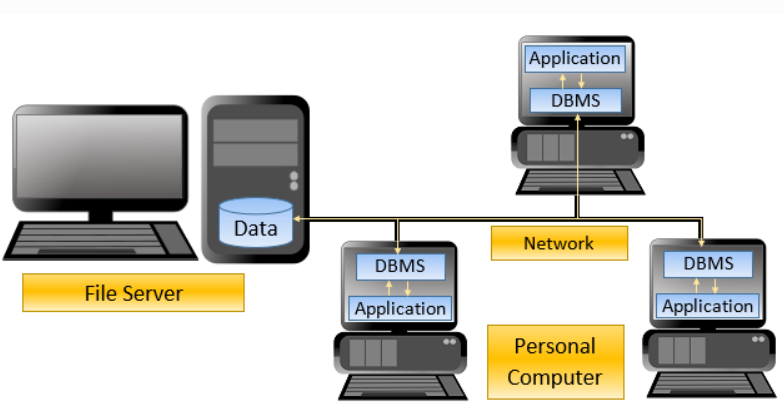
\includegraphics[height=0.3\textheight]{img/filesever} % height
	\caption{Архитектура файл-сервер \cite{architec}}
	\label{img:filesever}
\end{figure}
\subsubsection{Клиент-серверные}
Клиент-серверная СУБД располагается на сервере вместе с БД и осуществляет доступ к БД непосредственно, в монопольном режиме.
Клиентом (front end) является запрашивающая машина, сервером (back end) --- машина,
которая отвечает на запрос.
Характерной особенностью архитектуры клиент-сервер является перенос вычислительной нагрузки на сервер базы данных.
Особенно при выполнении запроса в базе данных по заданному пользователем запросу, так как клиентскому приложению посылается результат выполнения запроса, по сети путешествуют только те данные, которые необходимы клиенту. В итоге снижается нагрузка на сеть.
Результат выполнения запроса, который на несколько порядков меньше по объему, чем весь база данных (как в архитектуре файл-сервер), возвращается клиенту,
после чего интерпретирует его необходимым образом и представляет пользователю.

На рисунке \ref{img:clientsever} приведена клиент-серверная архитектура.

\begin{figure}[h!]
	\centering
	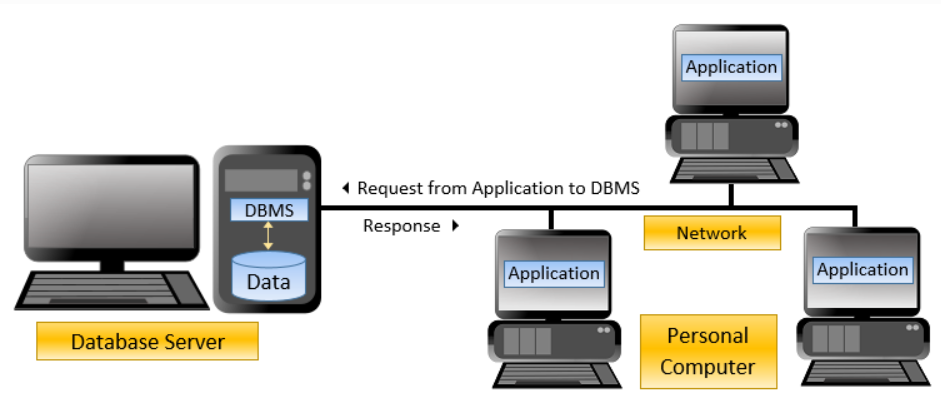
\includegraphics[height=0.25\textheight]{img/clientsever} % height
	\caption{Архитектура клиент-сервер \cite{architec}}
	\label{img:clientsever}
\end{figure}

База данных в этом случае помещается на сетевом сервере, как и в архитектуре файл-сервер, однако прямого доступа к базе данных из приложений не происходит.
Функцию прямого обращения к базе данных осуществляет СУБД.

Архитектура клиент-серверная имеет следующие преимущества \cite{classichoose}:
\begin{itemize}
	\item уменьшается сетевой трафик;
	\item уменьшается сложность клиентских приложений.
\end{itemize}

Однако у такой архитектуры есть несколько недостатков \cite{classichoose}:
\begin{itemize}
	\item могут быть трудности с обновлением программного обесппечения на клиентах;
	\item высокая стоимость оборудования.
\end{itemize}

\subsubsection{Встраиваемые}
Встраиваемая СУБД --- СУБД, которая может поставляться как составная часть
некоторого программного продукта, не требуя процедуры самостоятельной
установки. Характер этой архитектуры допускает работу сотен или даже тысяч одновременных пользователей. Поскольку по сети передается минимум данных, он подходит для сред, где быстрые и недорогие сетевые соединения остаются недоступными. Встраиваемая СУБД предназначена для локального хранения данных
своего приложения и не рассчитана на коллективное использование в сети.
Физически встраиваемая СУБД чаще всего реализована в виде подключаемой
библиотеки. Доступ к данным со стороны приложения может происходить через
SQL либо через специальные программные интерфейсы.
Встраиваемые СУБД быстрее обычных клиент-серверных и не требуют установки
сервера, поэтому востребованы в локальном программном обеспечении, которое имеет дело с большими объемами данных.

На рисунке \ref{img:inline} приведена встраиваемая архитектура.

\begin{figure}[h!]
	\centering
	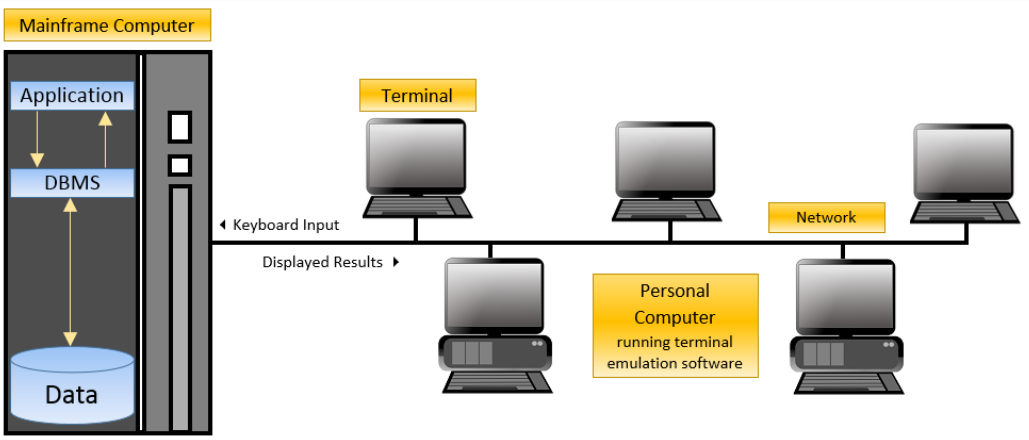
\includegraphics[height=0.25\textheight]{img/inline} % height
	\caption{Архитектура встраиваемая \cite{architec}}
	\label{img:inline}
\end{figure}

Встраиваемая архитектура имеет следующие преимушества \cite{classichoose}:
\begin{itemize}
	\item легкость разработки и развертывания приложений;
	\item легкость обслуживания локальной БД;
	\item высокое быстродействие на операциях считывания и модификации одиночных записей.
\end{itemize}

Однако у такой архитектуры есть несколько недостатков \cite{classichoose}:
\begin{itemize}
	\item высокий риск потери или повреждения данных;
	\item невозможность распределения вычислительной нагрузки.
\end{itemize}

\subsection{Критерии сравнения архитектур}
В данном разделе описаны критерии, которые используются для сравнения рассмативаемых архитектр в таблице \ref{tb:criteria}.

\begin{table}[ht]
	\begin{center}
		\begin{threeparttable}
			\caption{\label{tb:criteria}Критерии сравнения архитектур СУБД}
			\begin{tabular}{|c|p{8cm}|}
				\hline
				\textbf{Критерий} & \textbf{Описание} \\ \hline
				\textbf{Безопасность} & Включая различные политики управления пользователями и контроля доступа к данным \\ \hline
				\textbf{Скорость разработки} & Является ли архитектура быстрым в разработке \\ \hline
				\textbf{Производительность} & Выполняются запросы с высокой скоростью и эффективностью  \\ \hline
				\textbf{Гибкость} & Определяет степень, до которой система может быть легко адаптирована \\ \hline
				\textbf{Простота эксплуатации} & Оценка пользовательского интерфейса, документации и ресурсов поддержки \\ \hline
				\textbf{Стоимость} & Внедрения и использования, включая лицензионные сборы, расходы на обслуживание и любые дополнительные затраты \\ \hline
			\end{tabular}
		\end{threeparttable}
	\end{center}
\end{table}
\clearpage
\subsection{Сравнение архитектур СУБД}
\begin{table}[ht]
	\begin{center}
		\begin{threeparttable}
			\caption{\label{tab:comparison_1} Сравнение архитектур СУБД}
			\begin{tabular}{|c|c|c|c|}
				\hline
				\textbf{Критерий}            	& \textbf{Файл-сервер} 			 & \textbf{Клиент-сервер}    & \textbf{Встр-мая} \\ \hline
				\textit{Производительность}  	& \cmark/\xmark		 & \cmark 			& \cmark 			\\ \hline
				\textit{Безопасность}        	& \xmark 		   			 & \cmark 			& --- 			\\ \hline
				\textit{Скорость разработки} 	& \cmark 			 & \cmark/\xmark 				    & \cmark 			\\ \hline
				\textit{Гибкость}            	& \cmark/\xmark 	     & \cmark 			& --- 			\\ \hline
				\textit{Простота эксплуатации} & \cmark 		   			 & \cmark/\xmark 			& \cmark 			\\ \hline
				\textit{Стоимость} 				& \cmark			&\cmark/\xmark						&\cmark				\\ \hline
			\end{tabular}
		\end{threeparttable}
	\end{center}
\end{table}

Полученные результаты сводятся к следующему:
\begin{itemize}
	\item Файл-сервер --- самая низкая стоимость и эффиктивная в использовании и высокая скорость разработки. Однако она имеет ограниченную гибкость, особенно в масштабировании, так же низкую безопасность  и среднюю производительность.
	\item Клиент-сервер --- самая гибкая архитектура, вторая по производительности и самая безопасность с возможностью централизованного управления доступом. Однако она имеет сложность в разработке а также среднюю протстоту эксплуатации, так как требует более высокого уровня управления. Также, такая архитектура требует большие затраты на обслуживание и конфигурацию сервера.
	\item Встраиваемая --- самая высокая по производительности, так как интегрирована напрямую в приложение. Также, она имеет высокую скорость разработки и легкость в эксплуатации и низкую стоимость. Ее безопасность  зависит от функций, предоставленных встроенной СУБД, её гибкость зависит от функциональности встроенной СУБД.
\end{itemize}